\section{Architecture}
In this section the architecture of the plant monitoring system application will be described. All the following steps will be made by using the guide developed by Laurent Deru, Sébastien Dawans and Mathieu Ocana, available in GitHub under permissive 3-clause BSD-style open source license \cite{6lbr}. However, in the tutorial the TelosB node is used instead of the Texas Instrument Sensor Tags. Using the TI nodes is the overall greatest challenge described in this paper. Especially where the Sensor Tag is a relatively new node.\\
\subsection{The network}
The network main idea is well depicted in figure \ref{fig:Network}. The raspberry pi act as a six low pan border router (6LBR) and act as a link between the Ethernet and the wireless sensor network. The wireless sensor network is composed by the TelosB that act as a sink for all the other sensor tags. The TelosB sensor is attached via USB to the Raspberry Pi.
\begin{figure}[!h]
	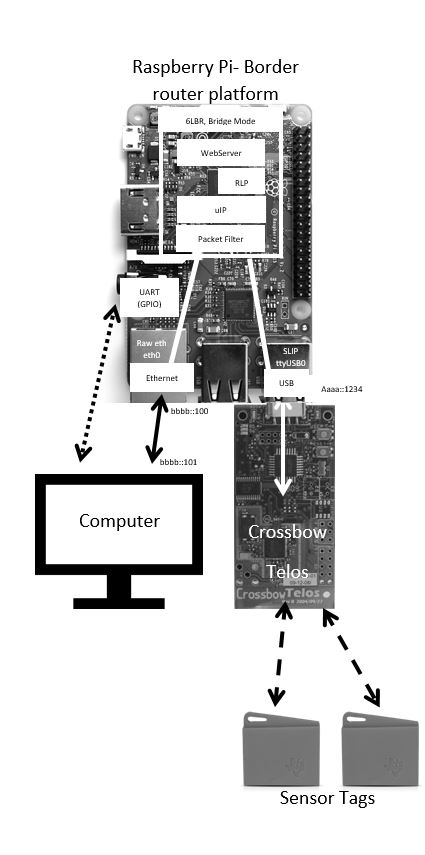
\includegraphics[width=\linewidth]{Network}
	\caption{Development of the network}
	\label{fig:Network}
\end{figure}
On the other hand, the Raspberry Pi is connected to a computer via a normal house router.
The Raspberry Pi connect the two subnets via RPL protocol on the wireless sensor network side and NPD on the Ethernet part.\\

\subsection{CoAP}
Before commence the description of web server, it is essential to explain the CoAP protocol. CoAP stands for Constarined Application Protocol \cite{coap}. It is an application protocol used for transferring information as it were HTTP, using the usual commands e.g. GET, PUT and POST. It works as client/server model where a server (in our case the sensor tag) can be requested to send data from the client side using the commands HTTP/CoAP commands. However, it differs from HTTP were CoAP works on constrained devices such as our sensor tag. CoAP is designed to limit the consumption of RAM, thus packets are made much smaller.

\subsection{WebServer}




